\documentclass[a4paper,12pt]{report}

\usepackage[utf8x]{inputenc}
\usepackage[T2A]{fontenc}
\usepackage[english, russian]{babel}
\usepackage[table]{xcolor}

% Опционно, требует  apt-get install scalable-cyrfonts.*
% и удаления одной строчки в cyrtimes.sty
% Сточку не удалять!
% \usepackage{cyrtimes}

% Картнки и tikz
\usepackage{graphicx}
\usepackage{tikz}
\usetikzlibrary{snakes,arrows,shapes}


% Увы, поля придётся уменьшить из-за листингов.
\topmargin -1cm
\oddsidemargin -0.5cm
\evensidemargin -0.5cm
\textwidth 17cm
\textheight 24cm

\sloppy



% Оглавление в PDF
\usepackage[
bookmarks=true,
colorlinks=true, linkcolor=black, anchorcolor=black, citecolor=black, menucolor=black,filecolor=black, urlcolor=black,
unicode=true
]{hyperref}

% Для исходного кода в тексте
% \newcommand{\Code}[1]{\texttt{#1}}

% Некоторая русификация.
% \usepackage{misccorr} % Oh shi^W^W, оно не работает с report.
\usepackage{indentfirst}
\renewcommand{\labelitemi}{\normalfont\bfseries{--}}

% На дворе XXI век, но пакет listings всё ещё не пашет с русскими комментариями!

% Пакет listings для простой вставки исходников
% \usepackage{listings}
% Параметры оформления
% \lstset{
% showspaces=false,
% showtabs=false,
% frame=single,
% tabsize=4,
% basicstyle=\ttfamily,
% identifierstyle=\ttfamily,
% commentstyle=\itshape,
% stringstyle=\ttfamily,
% keywordstyle=\ttfamily,
% breaklines=true
% }
% Русский в комментариях.
% \lstset{escapebegin=\begin{cyr},escapeend=\end{cyr}}

\usepackage{ifthen}
\ifx\requestedLaTeXdate\undefined
\usepackage{array}
\else
\usepackage{array}[=2016-10-06]
\fi
%%
% Packages required by doxygen
\usepackage{fixltx2e}
\usepackage{calc}
\usepackage{doxygen}
\usepackage{graphicx}
\usepackage{makeidx}
\usepackage{multicol}
\usepackage{multirow}
\PassOptionsToPackage{warn}{textcomp}
\usepackage{textcomp}
\usepackage[nointegrals]{wasysym}
\usepackage{ifpdf,ifxetex}

% NLS support packages
\usepackage[T2A]{fontenc}
\usepackage[russian]{babel}

% Font selection
\usepackage[T1]{fontenc}
\usepackage[scaled=.90]{helvet}
\usepackage{courier}
\usepackage{amssymb}
\usepackage{sectsty}
\renewcommand{\familydefault}{\sfdefault}
\allsectionsfont{%
  \fontseries{bc}\selectfont%
  \color{darkgray}%
}
\renewcommand{\DoxyLabelFont}{%
  \fontseries{bc}\selectfont%
  \color{darkgray}%
}
\newcommand{\+}{\discretionary{\mbox{\scriptsize$\hookleftarrow$}}{}{}}

% Arguments of doxygenemoji:
% 1) ':<text>:' form of the emoji, already "LaTeX"-escaped
% 2) file with the name of the emoji without the .png extension
% in case image exist use this otherwise use the ':<text>:' form
\newcommand{\doxygenemoji}[2]{%
  \IfFileExists{./#2.png}{\raisebox{-0.1em}{\includegraphics[height=0.9em]{./#2.png}}}{#1}%
}
% Page & text layout
\usepackage{geometry}
\geometry{%
  a4paper,%
  top=2.5cm,%
  bottom=2.5cm,%
  left=2.5cm,%
  right=2.5cm%
}
\tolerance=750
\hfuzz=15pt
\hbadness=750
\setlength{\emergencystretch}{15pt}
\setlength{\parindent}{0cm}
\newcommand{\doxynormalparskip}{\setlength{\parskip}{3ex plus 2ex minus 2ex}}
\newcommand{\doxytocparskip}{\setlength{\parskip}{1ex plus 0ex minus 0ex}}
\doxynormalparskip
\makeatletter
\renewcommand{\paragraph}{%
  \@startsection{paragraph}{4}{0ex}{-1.0ex}{1.0ex}{%
    \normalfont\normalsize\bfseries\SS@parafont%
  }%
}
\renewcommand{\subparagraph}{%
  \@startsection{subparagraph}{5}{0ex}{-1.0ex}{1.0ex}{%
    \normalfont\normalsize\bfseries\SS@subparafont%
  }%
}
\makeatother

\makeatletter
\newcommand\hrulefilll{\leavevmode\leaders\hrule\hskip 0pt plus 1filll\kern\z@}
\makeatother

% Headers & footers
\usepackage{fancyhdr}

% Indices & bibliography
\usepackage{natbib}
\usepackage[titles]{tocloft}
\setcounter{tocdepth}{3}
\setcounter{secnumdepth}{5}
\makeindex

\usepackage{newunicodechar}
  \newunicodechar{⁻}{${}^{-}$}% Superscript minus
  \newunicodechar{²}{${}^{2}$}% Superscript two
  \newunicodechar{³}{${}^{3}$}% Superscript three

% Custom commands
\newcommand{\clearemptydoublepage}{%
  \newpage{\pagestyle{empty}\cleardoublepage}%
}

\usepackage{caption}
\captionsetup{labelsep=space,justification=centering,font={bf},singlelinecheck=off,skip=4pt,position=top}

\usepackage{etoc}
\etocsettocstyle{\doxytocparskip}{\doxynormalparskip}
\renewcommand{\numberline}[1]{#1~}


\title{Расчетно-Пояснительная Записка \\ 
    \large к курсовой работе на тему: \\ Серверная часть MTA SMTP}
\author{Назаренко Никита Вадимович}

\begin{document}

\maketitle


\tableofcontents

\newpage
\addcontentsline{toc}{chapter}{Введение}
\chapter*{Введение}

Данная расчетно-пояснительная записка содержит информацию о протоколе SMTP (англ. \textbf{S}imple \textbf{M}ail \textbf{T}ransfer \textbf{P}rotocol) и реализации серверной части MTA (англ. \textbf{M}essage \textbf{T}ransfer \textbf{A}gent) SMTP в рамках курсового работа.

Задание: необходимо было создать SMTP-сервер, как часть MTA, обеспечивающий локальную доставку сообщений и их добавление в очередь удаленной доставки для клиента. Дополнительные условия:
\begin{itemize}
\item Используется poll;
\item Используется единственный рабочий поток;
\item Журналирование в отдельном процессе.
\end{itemize}

Цель работы: реализовать серверную часть MTA SMTP.

Основные задачи:
\begin{enumerate}
    \item Анализ и изучение протокола SMTP, способов мультиплексирования;
    \item Программная реализация SMTP сервера на языке программирования Си под Unix-подобные операционные системы;
    \item Тестирование и отладка написанного сервера;
    \item Оформление расчетно-пояснительной записки по результатам работы.
\end{enumerate}


\chapter{Аналитический раздел}


\section{Протокол SMTP}

SMTP (англ. \textbf{S}imple \textbf{M}ail \textbf{T}ransfer \textbf{P}rotocol) ~-- это широко используемый сетевой протокол, предназначенный для передачи писем электронной почты в сетях TCP/IP. SMTP впервые был описан в RFC 821 (1982 год), а последнее обновление описано в RFC 5321 (2008 год) и включает масштабируемое расширение протокола — ESMTP (Extended SMTP). В настоящее время под протоколом SMTP подразумеваются и его расширения. Протокол SMTP предназначен для передачи исходящей почты с использованием порта TCP 25.

Взаимодействие в рамках SMTP строится по принципу двусторонней связи, которая устанавливается между отправителем и получателем почтового сообщения. При этом отправитель инициирует соединение и посылает запросы, а получатель - отвечает на эти запросы. Таким образом, отправитель выступает в роли клиента, а получатель - сервера.


\subsection{Базовые команды SMTP}

Каждая команда SMTP начинается с ключевого слова – названия команды, указывающего какую операцию хочет произвести клиент. За ним могут следовать параметры, отделенные пробелом. Конец строк в протоколе SMTP обозначается последовательностью символов "возврат каретки"\ (\textbackslash r) и "перевод строки"\ (\textbackslash n) - эта последовательность обозначается CRLF. Сервер начинает выполнение команды только получив от клиента строку, завершающуюся последовательностью CRLF. 

Обычный ответ SMTP сервера на команды клиента состоит из номера ответа, за которым через пробел следует дополнительный текст. Номер ответа служит индикатором состояния сервера и делится на четыре группы:
\begin{itemize}
    \item Команда выполнена успешно (код 2xx);
    \item ромежуточный положительный результат. Команда принята, но сервер ожидает от клиента дополнительные данные для завершения операции (код 3xx);
    \item Исполнение команды временно невозможно. Команда не может быть выполнена, но проблема может быть устранена (код 4xx);
    \item Исполнение команды невозможно (код 5xx).
\end{itemize}

Если ответ состоит из нескольких строк, то каждая из них начинается номером, который отделяется от сопровождающего текста не пробелом, а символом "минус"\ (-). В последней строке номер отделяется от текста пробелом. Каждая строка ответа, как и строки команд, заканчивается последовательностью CRLF.

Ниже представлен список базовых SMTP-команд:
\begin{itemize}
    \item EHLO доменное\_имя\_клиента CRLF - Открывает ESMTP сессию. В ответ на эту команду сервер сообщает, готов ли он к продолжению диалога.
    \item HELO доменное\_имя\_клиента CRLF - Открывает SMTP сессию. В RFC 2821 рекомендуется использовать команду HELO, только если программное обеспечение не поддерживает команду EHLO. Отличие этой команды только в том, что она делает невозможным использование расширений ESMTP. Передача почты возможна только после выполнения одной из двух перечисленных выше команд.
    \item MAIL FROM: <адрес\_отправителя> CRLF - Сообщает адрес отправителя письма. Для каждого письма команда MAIL должна быть выполнена только один раз. Адрес может быть оставлен пустым: <>. Команда MAIL может быть выполнена только после успешного выполнения команды EHLO или HELO.
    \item RCPT TO: <адрес\_получателя> CRLF - Сообщает адрес получателя письма. Доставка сообщения возможна, только если указан хотя бы один адрес получателя. Команда RCPT принимает в качестве аргумента только один адрес. Если нужно послать письмо большему числу адресатов, то команду RCPT следует повторять для каждого. Команда RCPT может быть выполнена только после успешного выполнения команды MAIL.
    \item DATA CRLF - Определяет начало письма. C помощью этой команды серверу передается текст сообщения, состоящий из заголовка и отделенного от него пустой строкой тела сообщения. В ответ на правильно введенную команду DATA сервер сообщает о готовности к приему или об ошибке, если прием сообщения невозможен. Передача самого сообщения заканчивается строкой, состоящей из одной точки. Эта строка не является частью сообщения и удаляется на приемной стороне. Команда DATA может быть выполнена только после успешного выполнения хотя бы одной команды RCPT.
    \item RSET CRLF - Сброс SMTP соединения. Команда RSET аннулирует все переданные до нее на сервер данные.
    \item VRFY CRLF - Проверяет наличия указанного в качестве аргумента почтового ящика.
    \item QUIT CRLF - Закрыть SMTP сессию. Командой QUIT клиент заканчивает диалог с сервером. Сервер посылает подтверждение и закрывает соединение. Получив это подтверждение, клиент тоже прекращает связь.
\end{itemize}

\section{Плюсы и минусы использования однопоточного подхода обработки подключений при помощи мультиплексирования и системного вызова poll()}

В рамках задания необходимо реализовать серверную часть MTA SMTP с использованием системного вызова \texttt{poll()} в единственном рабочем потоке. К плюсам данного подхода можно отнести:
\begin{itemize}
    \item Нет нужды создавать новые процессы или потоки, что является затратной операцией для ОС.
    \item Нет активного ожидания на процессоре.
    \item Все взаимодействие с сокетами осуществляется в одном потоке выполнения, что снимает необходимость синхронизации доступа к разделяемым ресурсам.
    \item Позволяет обрабатывать больше 1024 клиентов по сравнению с системным вызовом \texttt{select()}.
\end{itemize}

К минусам использования этого подхода относятся:
\begin{itemize}
    \item Усложняется работа с памятью, так как \texttt{poll()} может потребовать использование динамических массивов.
    \item В полностью однопоточном подходе может увеличится время обработки каждого подключения при больших количествах активных соединений по сравнению с подходом в несколько потоков.
\end{itemize}


\section{Сущности предметной области}

Для SMTP сервера можно выделить две основные сущности, которыми необходимо оперировать (обрабатывать, сохранять):
\begin{enumerate}
    \item Клиент - текущее активное соединение с информацией о подключении (буферы ввода-вывода, длина, состояние)
    \item Письмо - передаваемое клиентом сообщение на сервер с заголовками (отправитель, получатель, тема и т.д.) и данными (сам текст письма).
\end{enumerate}


\chapter{Конструкторский раздел}


\section{Конечный автомат состояний сервера}

На рис.~\ref{fig:fsm} изображен конечный автомат состояний серверной части MTA SMTP. 

\begin{figure}[h]
    \centering
    \includegraphics[width=\textwidth]{include/server_def_dot.pdf}
    \caption{Конечный автомат состояний сервера}
    \label{fig:fsm}
\end{figure}

Как можно заметить, команды, связанные с отправкой сообщения (например, MAIL), могут обрабатываться только после вызова HELO или EHLO. Соответственно RCPT может вызываться только после MAIL, а DATA только после RCPT. После вызова DATA ожидается окончание письма, для его сохранения и записи. По остальным командам особых ограничений не имеется. 

В случае продолжительного бейздействия клиента (ничего не отправляется заданное заранее время), сервер обрывает соединение по таймауту с уведомлением об этом клиента.


\section{Синтаксис команд протокола}

Ниже приведены регулярные выражения всех использующихся команд протокола и вспомогательные регулярные выражения, использующиеся в них:
\begin{description}
    \item[Возможные символы пробела]
    \input{include/spaces_regexp.tex}
    \item[Домен]
    \input{include/domain_regexp.tex}
    \item[Почтовый адрес]
    \input{include/address_regexp.tex}
    \item[Почтовый адрес или пустой адрес]
    \input{include/address_or_empty_regexp.tex}
    \item[Конец строки (CLRF)]
    \textbackslash r\textbackslash n
    \item[Команда HELO]
    \input{include/helo_cmd_regexp.tex}
    \item[Команда EHLO]
    \input{include/ehlo_cmd_regexp.tex}
    \item[Команда MAIL]
    \input{include/mail_cmd_regexp.tex}
    \item[Команда RCPT]
    \input{include/rcpt_cmd_regexp.tex}
    \item[Команда DATA]
    \input{include/data_cmd_regexp.tex}
    \item[Команда RSET]
    \input{include/rset_cmd_regexp.tex}
    \item[Команда VRFY]
    \input{include/vrfy_cmd_regexp.tex}
    \item[Команда QUIT]
    \input{include/quit_cmd_regexp.tex}
\end{description}


\section{Описание основных структур данных}

На рис.~\ref{fig:er} изображены основные структуры данных сервера, а именно:
\begin{itemize}
    \item Server - абстракция сервера, содержащая в себе словарь клиентов, дескрипторы их сокетов и таймауты, а также справочную информацию (доменное имя сервера, пути до папок с письмами).
    \item Client dictionary - словарь клиентов. В качестве ключа используется номер файлового дескриптора сокета клиента.
    \item Client - абстракция клиента, содержащая в себе буферы ввода-вывода, их длины, текущее состояние подключения клиента и текущее письмо.
    \item Mail - абстракция письма. Состоит из полей отправителя, данных (текста письма), массива получателей, их количества и типа (получатели только локальные, только удаленные или оба).
\end{itemize}

\begin{figure}[h]
    \centering
    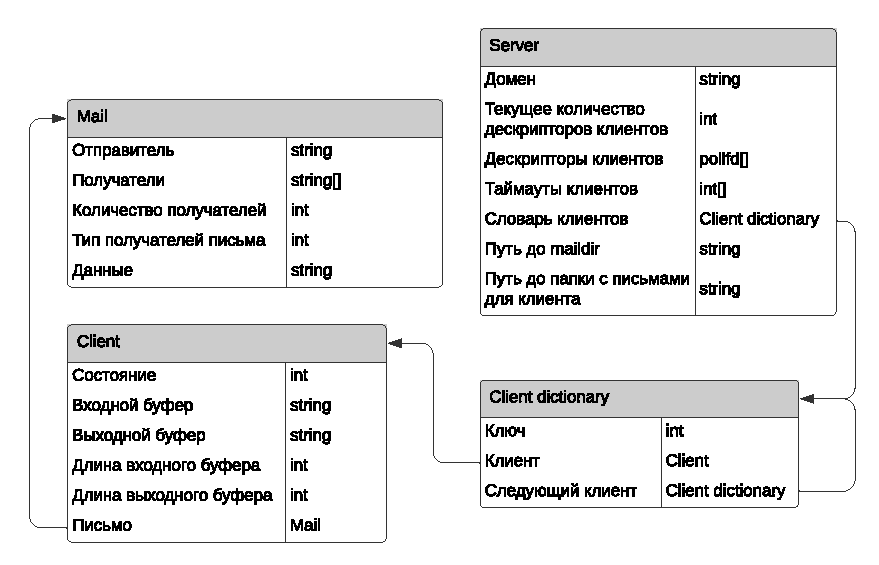
\includegraphics[width=\textwidth]{pics/er.pdf}
    \caption{ER-диаграмма основных структур данных}
    \label{fig:er}
\end{figure}


\section{Обработка соединений в одном потоке выполнения}

Ниже представлен псевдокод обработки сервером клиентских соединений в одном потоке выполнения:

\begin{verbatim}
    Если пришло сообщение в файловый дескриптор для выхода
        Выйти
    
    Если пришло сообщение на сокет сервера 
        Обработать новое подключение и добавить нового клиента
    
    Цикл по всем дескрипторам сокетов клиента
        Если пришло сообщение на сокет клиента
            Обнулить таймер клиента
            Обработать сообщение от клиента
        Если нужно отправить сообщение клиенту
            Отослать сообщение клиенту

    Увеличить таймер всех клиентов на 1
    Если таймер клиента превысил определенное заданное значение
        Оборвать соединение с клиентом
\end{verbatim}


\section{Связь основной программы и процесса журналирования}

На рис.~\ref{fig:ipc} изображена связь между основной программой и процессом журналирования с использованием очереди сообщений.

\begin{figure}[h]
    \centering
    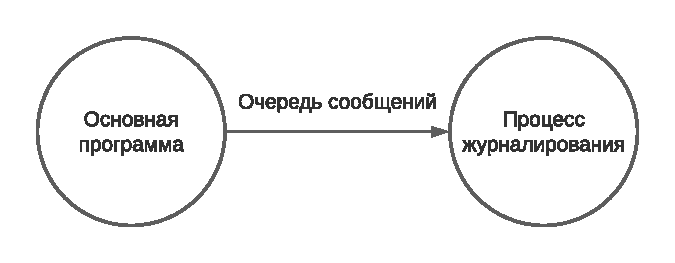
\includegraphics[width=0.7\textwidth]{pics/ipc.pdf}
    \caption{Связь основной программы и процесса журналирования}
    \label{fig:ipc}
\end{figure}


\section{Хранение почты}

Для хранения локальной почты, то есть предназначенной для клиентов с почтовым доменом сервера, используется упрощенный формат Maildir. Maildir - формат хранения электронной почты, не требующий монопольного захвата файла для обеспечения целостности почтового ящика при чтении, добавлении или изменении сообщений. Каждое сообщение хранится в отдельном файле с уникальным именем, а каждая папка представляет собой каталог. Вопросами блокировки файлов при добавлении, перемещении и удалении файлов занимается локальная файловая система. Все изменения делаются при помощи атомарных файловых операций, таким образом, монопольный захват файла ни в каком случае не нужен.

Для почты, предназначенной другим почтовым серверам также используется файловая система. Каждое сообщение аналогично хранится в отдельном файле с уникальным именем. Все файлы складываются в одну директорию, из которой в дальнейшем клиент считывает письма для их пересылки. 

Для того, чтобы имена файлов были уникальными, в их качестве используется формат Unix time (рус. Unix-время) - система описания моментов во времени, принятая в Unix и других POSIX-совместимых операционных системах. Определяется как количество секунд, прошедших с полуночи (00:00:00 UTC) 1 января 1970 года.


\chapter{Технологический раздел}


\section{Платформы и компиляторы}

Разработанное приложение SMTP сервера проверялось на операционной системе Ubuntu-20.04 в подсистеме WSL (англ. \textbf{W}indows \textbf{S}ybsystem \textbf{L}inux) с использованием компилятора GCC и стандарта языка Си C99.


\section{Сборка программы}

Сборка системы разделена на две части и описана в файлах \texttt{Makefile} системы сборки \texttt{make}.

Первая часть, верхнеуровневая, описывает описывает сборку всего MTA, включая и серверную часть и клиентскую. Однако также можно указать сборку только одной части. В данном файле указываются флаги для сборки сервера и клиента, а также директория, где будут лежать запускамые бирнарные файлы. В качестве аргумента при вызове \texttt{make} принимается параметр \texttt{build\_type}, который может быть равен \texttt{debug} или \texttt{release}. По умолчанию стоит \texttt{debug}. Пример вызовов:
\begin{verbatim}
    make server
    make build_type=release
\end{verbatim}

Вторая часть относится непосредственно к сборке приложения сервера и запуску тестов и вызывается из верхнеуровнего файла сборки. В этом файле указываются имя результирующего бинарного файла, флаги компилятора, линковщика и папки с исходным кодом программы. Все зависимости \texttt{make} ищет сам в рамках указанных папок.


\section{Основные функции программы}

Данный раздел сгеренерирован при помощи doxygen из части комментированных исходников программы. В файле конфигурации \textbf{doxyggen.cfg} был отключён параметр \textbf{HAVE\_DOT}, поскольку для рисования графов вызовов используется \textit{cflow}.

Здесь описываются основные функции сервера, отвечающие за его работоспособность.

\hypertarget{main_8c}{}\subsection{Файл main.\+c}
\label{main_8c}\index{main.\+c@{main.\+c}}


Main entry point file.  


\subsubsection*{Структуры данных}
\begin{DoxyCompactItemize}
\item 
struct \hyperlink{structoptions__struct}{options\+\_\+struct}
\begin{DoxyCompactList}\small\item\em Client options struct. \end{DoxyCompactList}\end{DoxyCompactItemize}
\subsubsection*{Определения типов}
\begin{DoxyCompactItemize}
\item 
typedef struct \hyperlink{structoptions__struct}{options\+\_\+struct} \hyperlink{main_8c_a30bf13acdd62b5624d37afb6f89a6e0c}{options\+\_\+t}\hypertarget{main_8c_a30bf13acdd62b5624d37afb6f89a6e0c}{}\label{main_8c_a30bf13acdd62b5624d37afb6f89a6e0c}

\begin{DoxyCompactList}\small\item\em Client options struct. \end{DoxyCompactList}\end{DoxyCompactItemize}
\subsubsection*{Функции}
\begin{DoxyCompactItemize}
\item 
static void {\bfseries close\+\_\+handler} (int signal)\hypertarget{main_8c_adafcb2d413890485316dc00bbd87d2f0}{}\label{main_8c_adafcb2d413890485316dc00bbd87d2f0}

\item 
int \hyperlink{main_8c_a859307c43da5908cb529781d87068c29}{main\+\_\+loop} ()\hypertarget{main_8c_a859307c43da5908cb529781d87068c29}{}\label{main_8c_a859307c43da5908cb529781d87068c29}

\begin{DoxyCompactList}\small\item\em Main client loop func. \end{DoxyCompactList}\item 
\hyperlink{main_8c_a30bf13acdd62b5624d37afb6f89a6e0c}{options\+\_\+t} {\bfseries fill\+\_\+options} ()\hypertarget{main_8c_a0fec7fc1601ea618067b662f02c512cf}{}\label{main_8c_a0fec7fc1601ea618067b662f02c512cf}

\item 
int {\bfseries validate\+\_\+options} (\hyperlink{main_8c_a30bf13acdd62b5624d37afb6f89a6e0c}{options\+\_\+t} options)\hypertarget{main_8c_ada9147964d2cd1be480dd27aae5294c7}{}\label{main_8c_ada9147964d2cd1be480dd27aae5294c7}

\item 
int {\bfseries main} (int argc, char $\ast$$\ast$argv)\hypertarget{main_8c_a3c04138a5bfe5d72780bb7e82a18e627}{}\label{main_8c_a3c04138a5bfe5d72780bb7e82a18e627}

\end{DoxyCompactItemize}
\subsubsection*{Переменные}
\begin{DoxyCompactItemize}
\item 
static volatile int {\bfseries run} = 1\hypertarget{main_8c_a86d4c45d6f679f903dd72e84f4b961c8}{}\label{main_8c_a86d4c45d6f679f903dd72e84f4b961c8}

\item 
static logger\+\_\+t $\ast$ {\bfseries logger}\hypertarget{main_8c_a9575b06719f9ef5b9443b1dc68d38fe4}{}\label{main_8c_a9575b06719f9ef5b9443b1dc68d38fe4}

\item 
static int {\bfseries pipe\+Descrs} \mbox{[}2\mbox{]} = \{ 0, 0 \}\hypertarget{main_8c_affb0b2f4ce744f48e98e0a8aad5b673a}{}\label{main_8c_affb0b2f4ce744f48e98e0a8aad5b673a}

\item 
\hyperlink{main_8c_a30bf13acdd62b5624d37afb6f89a6e0c}{options\+\_\+t} {\bfseries client\+\_\+options}\hypertarget{main_8c_a0b3ee24a66a4de50f4d5714869d1231b}{}\label{main_8c_a0b3ee24a66a4de50f4d5714869d1231b}

\end{DoxyCompactItemize}


\subsubsection{Подробное описание}
Main entry point file. 


\input{include/server_8h.tex}


\section{Основные структуры программы}

Данный раздел также как и прошлый сгеренерирован при помощи doxygen и описывает основные структуры, использующиеся в коде сервера и на которые ссылаются его основные функции.

\input{include/structserver__struct.tex}
\input{include/structserver__client__dict__struct.tex}
\input{include/structserver__client__struct.tex}
\input{include/structmail__struct.tex}


\section{Описание параметров командной строки}

Ниже приведено описание используемых сервером параметров командной строки в формате autoopts:

AutoGen Definitions options;
prog-name     = server;
prog-title    = "SMTP server";
long-opts;
gnu-usage;    /* GNU style preferred to default */

flag = {
    name      = port;           /* Порт, который слушает сервер */
    value     = p;              /* Краткий флаг (-p) */
    arg-type  = number;
    arg-range = 110;
    arg-range = "1024->65000";
    max       = 1;              /* Не более одного раза */
    min       = 1;              /* Обязательный параметр */
    descrip   = "Port to bind";
};

flag = {
    name      = log_dir;        /* Путь до директории с лог-файлами */
    value     = l;              /* Краткий флаг (-l) */
    arg-type  = string;
    max       = 1;              /* Не более одного раза */
    min       = 0;              /* Необязательный параметр */
    descrip   = "Path to the log directory";
};

flag = {
    name      = mail_dir;       /* Путь к директории с локальными письмами */
    value     = d;              /* Краткий флаг (-d) */
    arg-type  = string;
    max       = 1;              /* Не более одного раза */
    min       = 0;              /* Необязательный параметр */
    descrip   = "Path to the maildir directory";
};


\section{Графы вызова функций}

Графы вызова функций разбиты на два рисунка. На рис.~\ref{fig:cflow1} показаны основные функции, связанные с работоспособностью сервера. На рис.~\ref{fig:cflow2} в свою очередь показаны функции обработки команд и конечного автомата состояний сервера.

\begin{figure}[h]
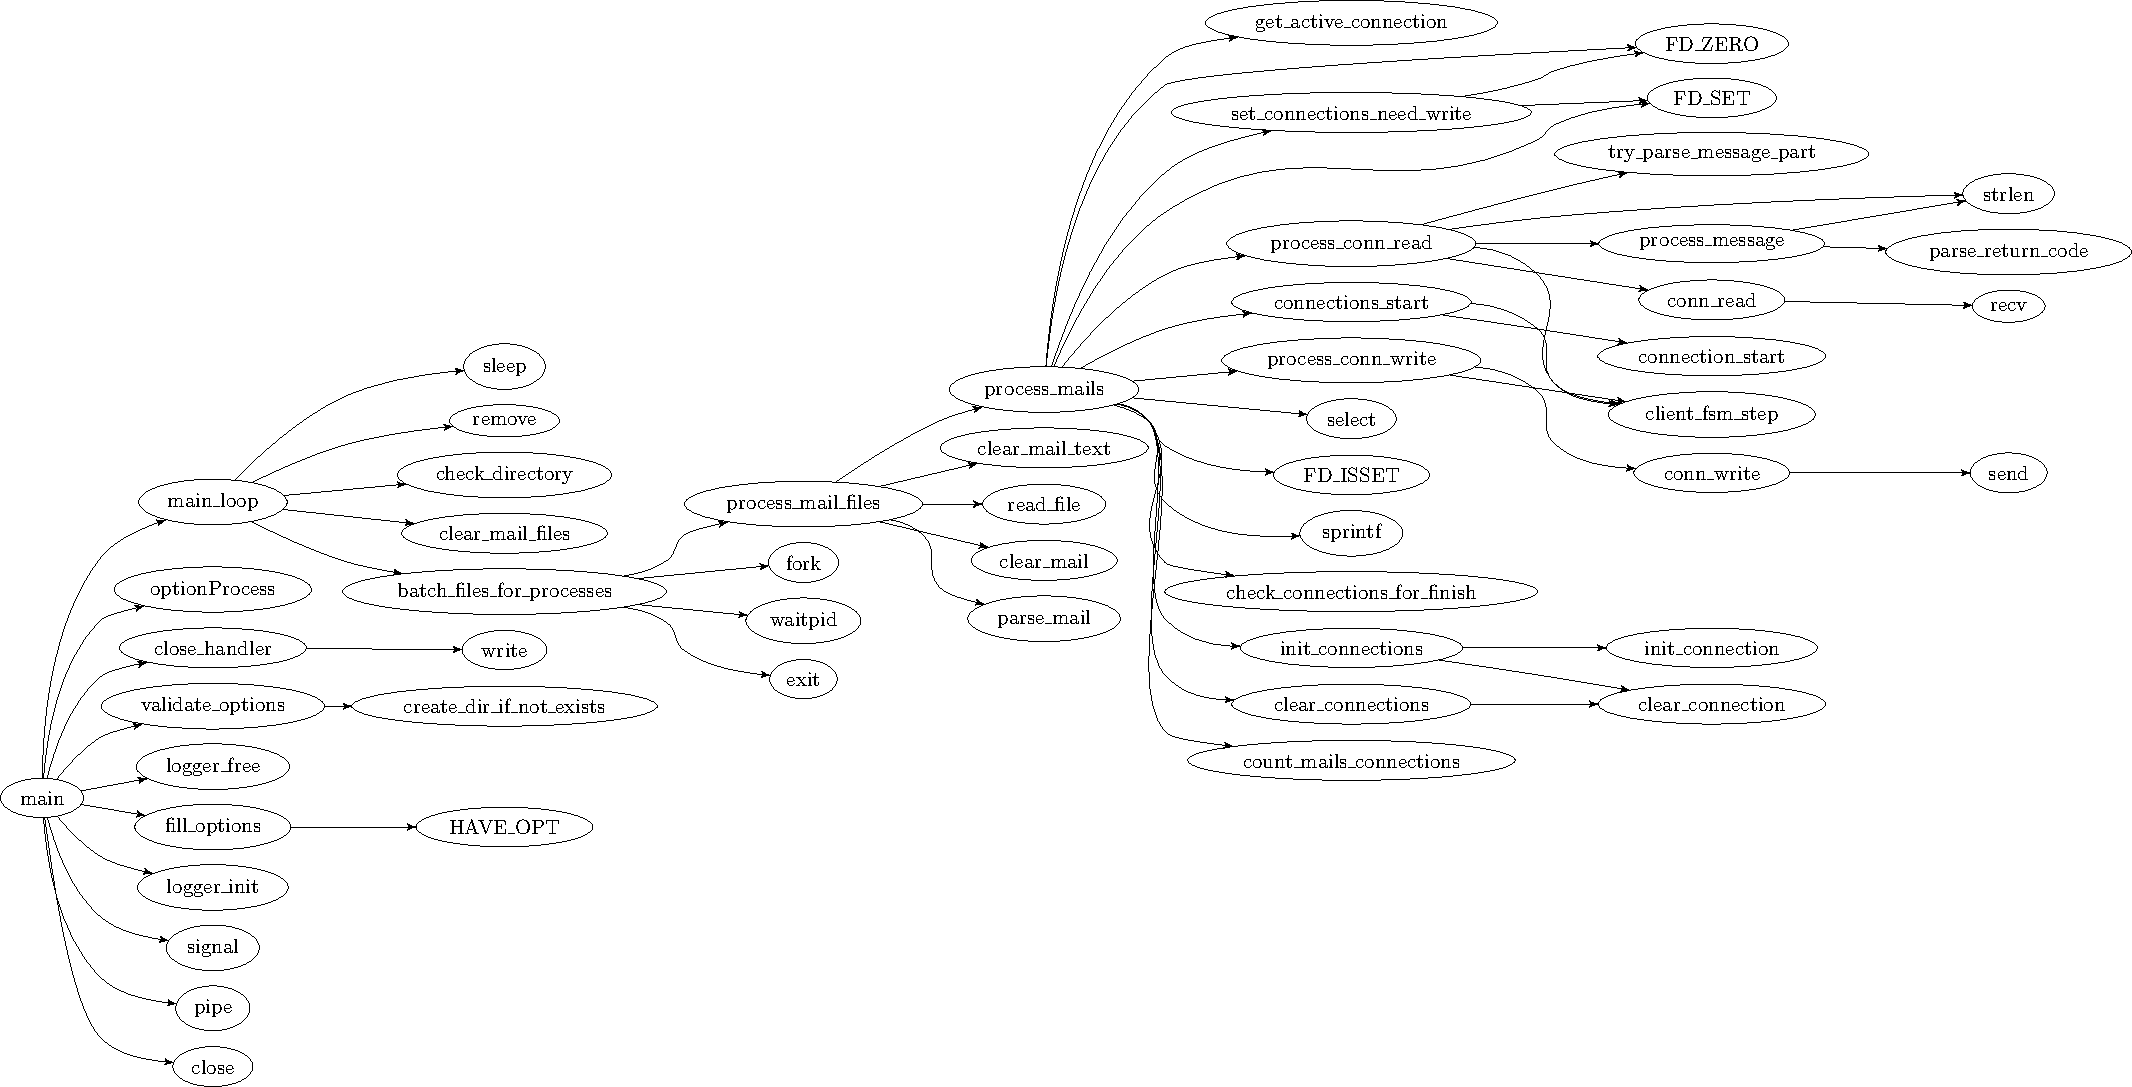
\includegraphics[width=1.1\textwidth]{include/cflow_main_dot.pdf}
\caption{Граф вызовов. Основные функции}
\label{fig:cflow1}
\end{figure}

\begin{figure}[h]
\centering
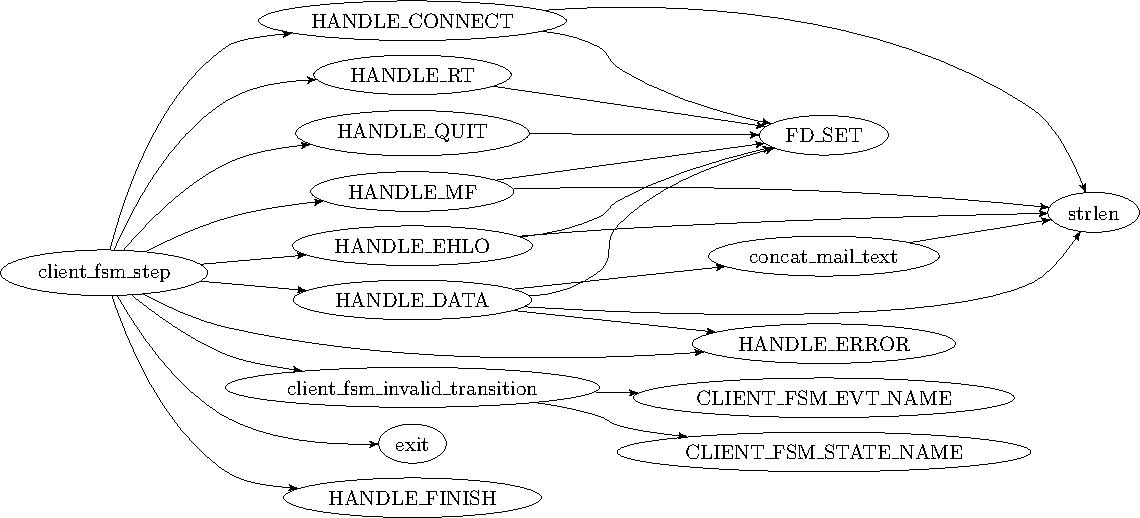
\includegraphics[width=\textwidth]{include/cflow_handlers_dot.pdf}
\caption{Граф вызовов. Функции обработки команд}
\label{fig:cflow2}
\end{figure}

Сами графы были созданы с помощью \texttt{cflow}, \texttt{cflow2dot} и \texttt{dot}.


\section{Модульное тестирование}

Для модульного тестирования функций сервера в работе используется библиотека CUnit. Тестировались все основные модули, такие как: модуль писем, клиентов, парсера команд, сервера и обработчика команд от клиента. Ниже приведены сводные результаты тестирования:
\begin{verbatim}
    Run Summary:    Type  Total    Ran Passed Failed Inactive
              suites      5      5    n/a      0        0
               tests     21     21     21      0        0
             asserts     87     87     87      0      n/a

    Elapsed time =    0.011 seconds
\end{verbatim}


\section{Системное тестирование}




\section{Тестирование утечек памяти}




\newpage
\addcontentsline{toc}{chapter}{Заключение}
\chapter*{Заключение}

В процессе выполнения работы была написана программная реализация серверной части MTA SMTP. Был изучен протокол передачи электронной почты SMTP и способы мультиплексирования. Были закреплены и получены навыки в написании сетевых приложений на языке Си для Unix-подобных операционных систем. Было проведено тестирование и отладка разработанного серверного приложения и в итоге по результатам проведенной работы была оформлена расчетно-пояснительная записка.


\end{document}
